%\section{The RADIUS Approach}\label{sec:approach} 
\section{The RADIUS Techniques}\label{sec:approach} 

RADIUS aims to achieve robust and accurate detection for maintaining the network performance by combining the Bayesian thresholding with several supporting techniques. 
%In addition, to further increase the accuracy and robustness of RADIUS and enable its adaptiveness to dynamic environments, we introduce several auxiliary techniques. 
In this section, we present the Bayesian thresholding technique, elaborate the supporting techniques and identify the involved parameters. 

%RADIUS aims to achieve robust and accurate detection for maintaining the network performance by employing the Bayesian thresholding technique. In addition, to further increase the accuracy and robustness of RADIUS and enable its adaptiveness to dynamic environments, we introduce several auxiliary techniques. In this section, we present the Bayesian thresholding technique, elaborate the supporting techniques and identify the involved parameters. 

%\vspace{-0.05cm}
\subsection{Bayesian Thresholding} \label{sec:thdComputation}

A classical example that employs Bayesian thresholding is the binary detection problem, as known in the communication literature \cite{lee2012digital}. The goal is to detect binary digits ``0'' and ``1'' in a noisy channel based on the received signal level with the knowledge of the \textit{a priori} probabilities of ``0'' and ``1''. Mapping such a problem to our problem of detecting link quality degradation, our goal is to detect a link either being a good link (with low packet losses) or a weak link (with high packet losses) with a minimized error rate based on the RSSI values measured at the receiver of the link.

%\paragraph{Mathematic Basis.}
\paragraph{Mathematic Basis.} Let $H_g$ and $H_w$ respectively denote a link being a good and a weak link. Let $E$ denote a detection error (either a false positive or a false negative). Then, based on the Bayes decision theory, $P(E)$, the probability of detection error, can be expressed in terms of conditional probabilities as follows:
\setlength{\belowdisplayskip}{4pt} \setlength{\belowdisplayshortskip}{4pt}
\setlength{\abovedisplayskip}{4pt} \setlength{\abovedisplayshortskip}{4pt}
\begin{equation} \label{equ:bayesRule}
	P(E) = P(E|H_g)P(H_g) + P(E|H_w)P(H_w),
\end{equation}
where $P(H_g)$ is the \textit{a priori} probability of a link being a good link, and $P(H_w)=1-P(H_g)$. $P(E|H_g)$ is the probability of false positives, i.e., misidentifying a good link as a weak link, while $P(E|H_w)$ is the probability of false negatives, i.e., failing to detect a degradation in link quality. 

% --------------------------------------- 
We assume that the RSSI follows a normal distribution $N(\mu, \sigma)$,
%$\aleph(\mu, \sigma)$,
which has been experimentally validated for low power communication in WSNs \cite{7164923, Rappaport:1996:WCP:525688}. For simplicity, we further assume that the distributions of RSSI for a weak link and for a good link, while with different means  $\mu_w$ and $\mu_g$ respectively, have the same standard deviation $\sigma$. In other words, the probability density functions of RSSI for the good link $f_g(x)$ and for the weak link $f_w(x)$ are as follows:
\begin{eqnarray}
	f_g(x) &=& \frac{1}{\sqrt{2\pi}\sigma}exp\left\lbrace -(x-\mu_g)^2 / 2\sigma^2\right\rbrace \label{equ:pdfWeak} \\
	f_w(x) &=& \frac{1}{\sqrt{2\pi}\sigma}exp\left\lbrace -(x-\mu_w)^2 / 2\sigma^2\right\rbrace \label{equ:pdfGood}
\end{eqnarray}
An example of these density functions is plotted in Figure \ref{fig:rssi-threshold}, where the false positive rate and the false negative rate are marked as shaded areas with respect to an RSSI threshold $\tau$. 

\begin{figure}
	\centering
	%\vspace{-0.1cm}
	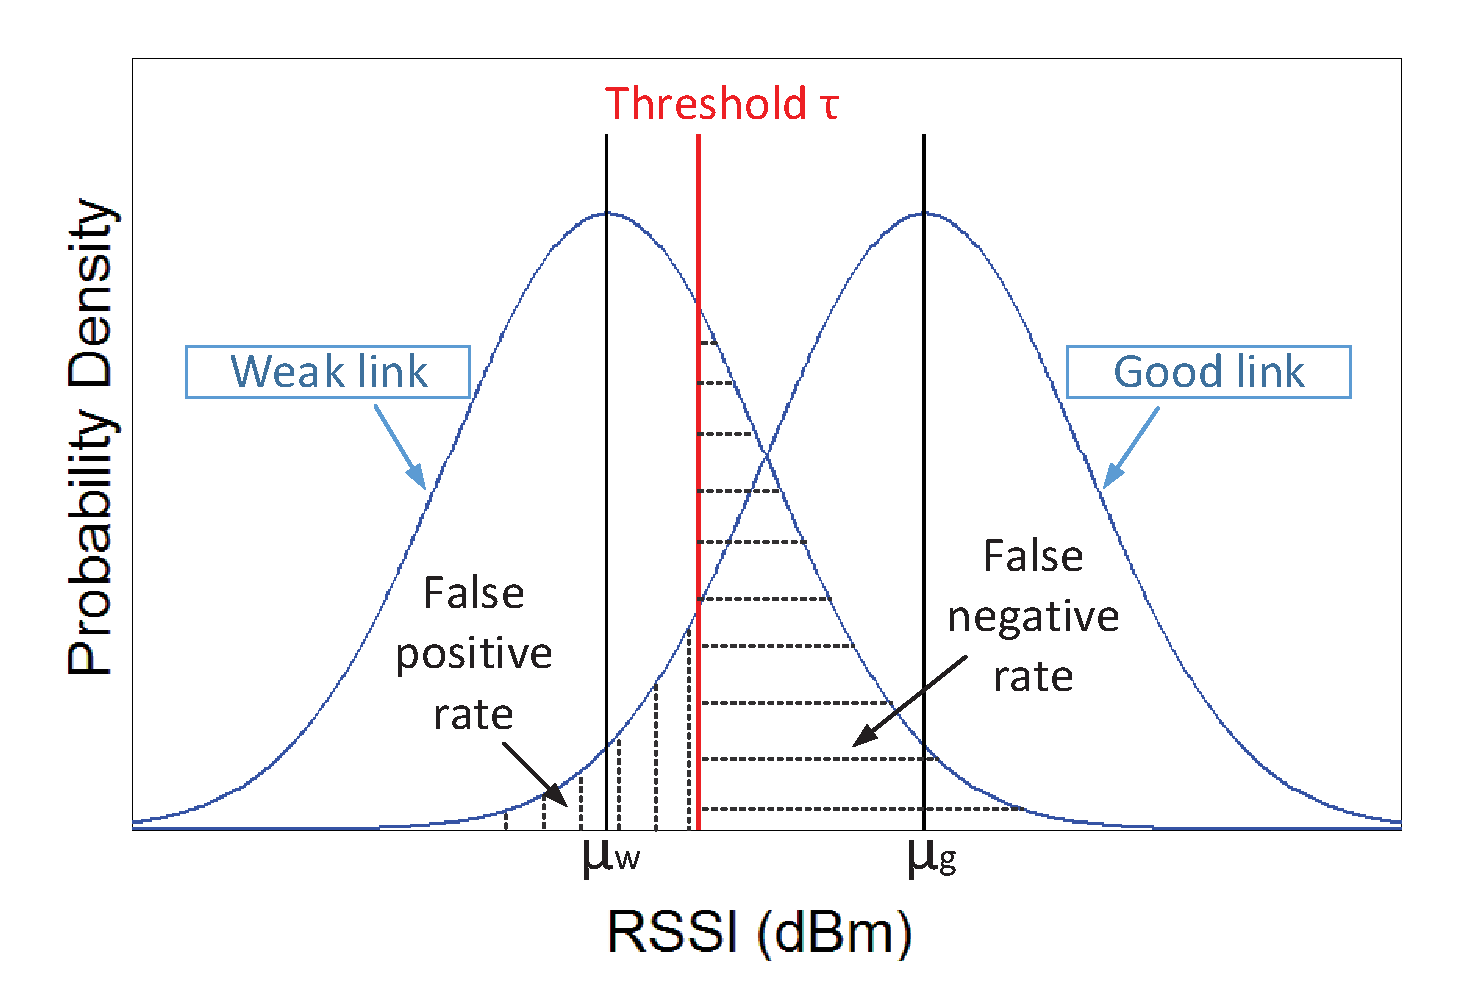
\includegraphics[width=1\linewidth]{rssi-threshold}
	\vspace{-0.8cm}
	\caption{\textbf{Illustration of the probabilities of error for a binary classification problem with Gaussian distribution.}}
	\label{fig:rssi-threshold}
	\vspace{-0.8cm}
\end{figure}

Based on Equations \ref{equ:pdfWeak} and \ref{equ:pdfGood}, the Bayes error $P(E)$ can be expressed as a function of the threshold $\tau$:
%\setlength{\belowdisplayskip}{4pt} \setlength{\belowdisplayshortskip}{4pt}
%\setlength{\abovedisplayskip}{4pt} \setlength{\abovedisplayshortskip}{4pt}
\begin{equation} \label{equ:fpr}
	P_E(\tau) = \int_{-\infty}^{\tau} f_g(x) dx \cdot P(H_g) + \int_{\tau}^{\infty} f_w(x) dx \cdot P(H_w)
\end{equation}

%\begin{equation} \label{equ:fpr}
%	P_E(\tau) = \int_{\tau}^{\infty} f_g(x) dx \cdot P(H_g) + \int_{-\infty}^{\tau} f_w(x) dx \cdot P(H_w)
%\end{equation}

%\vspace{-0.2cm}
We minimize $P(E)$ by letting $d\Big(P_E(\tau)\Big)/d\tau = 0$. We can then obtain the optimal threshold $T_{Bayes}$ that minimizes the detection error and the resultant Bayes error $P_E$ as follows:
\begin{align}  
	T_{Bayes} &= \frac{1}{2}(\mu_g + \mu_w) + \frac{\sigma^2 ln(P(H_w)/P(H_g))}{\mu_g - \mu_w} \label{equ:rssiTHD} \\
	P_E(\alpha) &= Q\bigg[\alpha - \frac{1}{2} \alpha^{-1} ln\Big(P(H_w)/P(H_g)\Big)\bigg]P(H_g) \nonumber \\
	& + Q\bigg[\alpha + \frac{1}{2} \alpha^{-1} ln\Big(P(H_w)/P(H_g)\Big)\bigg]P(H_w) \label{equ:error}   
\end{align} 
where $Q(x)$ is a Q-function \cite{wiki:qfunction} and $\alpha$ is defined as: 
%\setlength{\belowdisplayskip}{4pt} \setlength{\belowdisplayshortskip}{4pt}
%\setlength{\abovedisplayskip}{4pt} \setlength{\abovedisplayshortskip}{4pt}
\begin{equation} \label{equ:similarityMetric}
	\alpha = (\mu_g - \mu_w)/2\sigma. 
\end{equation}
%\vspace{-0.2cm}


%\subsubsection{Application to RADIUS}
\paragraph{Application to RADIUS.} Applying the Bayesian thresholding technique to RADIUS essentially requires to find the Bayes threshold $T_{Bayes}$, as computed in Equation \ref{equ:rssiTHD}. The use of Equation \ref{equ:rssiTHD} also indicates that the computation of the Bayes threshold only depends on a few statistical measures, significantly reducing the complexity in comparison to typical Bayesian decision problems. These statistical measures include the mean of the density distribution of RSSI for a good link and for a weak link ($\mu_{g}$ and $\mu_{w}$, respectively), as well as the standard deviation $\sigma$ of the distribution. 

In the RADIUS system, the VCC monitors the end-to-end packet delivery ratio (PDR) of the network after the network is deployed. When the PDR satisfies the minimal user requirements, implying that all links being used are good links, the VCC informs all DAs to start the training phase. During this phase, the statistical measures $\mu_{g}$ and $\sigma$ are computed from the collected RSSI samples for each individual link relevant to the higher-layer routing protocols. For the value of $\mu_{w}$, we choose the border RSSI value of the ``grey zone'' (i.e., $\mu_w = -88$ dBm) reported in previous experimental studies \cite{Lin:atpc, 7164923}, which show that PDR decreases significantly when a link enters the ``grey zone''. 

The \textit{a priori} probability $P(H_g)$ required in Equation \ref{equ:rssiTHD} is typically computed empirically based on previous experience or measurements. As this parameter has to be defined before the deployment, the setting of $P(H_g)$ impacts on the detection performance of the operational system. In Section \ref{sec:motivationBayes}, we have presented its effect on the detection error in general. In Section \ref{sec:ThresholdChoice}, we will quantify the effect of $P(H_g)$ on the FPR and the FNR in more details.


%\subsection{Supporting Techniques in RADIUS} \label{sec:supportingTechniques}
\paragraph{Bayesian thresholding alone is not enough.} Despite that the Bayes threshold is designed in RADIUS to minimize detection error, it alone is not enough to build a robust and accurate system for the detection of anomalous link quality degradation in WSNs. There are several inherent challenges that have to be addressed in order to apply the thresholding technique. Some of them are introduced by the technique itself (e.g., accurate estimation of $\mu_{g}$ and $\sigma$) while the others are caused by the fact that RSSI is highly influenced by environment changes (e.g., smoothing and threshold adaptation). In the rest of this section, we introduce these challenges and the techniques that we employ in RADIUS to address them.

%\subsubsection{To avoid high detection error due to insufficient training, we need to know how many RSSI samples are needed for a good enough approximation of the true underlying conditional distribution}
\subsection{Estimating the Minimal Training Set Size}\label{sec:minTrainingSet}
%%\textit{Problem 1: To avoid high detection error due to insufficient training, we need to know how many RSSI samples are needed for a good enough approximation of the true underlying conditional distribution.}

According to Equation \ref{equ:rssiTHD}, finding the Bayes threshold requires to compute the mean $\mu_{g}$ and the standard deviation $\sigma$ from a collected RSSI training set. The size of such a training set has a significant impact on the estimation error of $\mu_{g}$ and $\sigma$ and hence a great impact on the system detection accuracy. Deciding the training set size involves considering a tradeoff between the detection accuracy and the training latency. A larger training set can provide a more accurate estimation of the underlying data distribution thus higher accuracy in estimating $\mu_{g}$ and $\sigma$, while it may significantly increase the training time. In addition, the training size should also differ from link to link for the specific statistical characteristics of individual links: small training set size may suffice for a stable link while a larger size is required for links with highly fluctuating RSSI readings. 

%\textbf{Estimating the Minimal Training Set Size ($N_{ts}$) }. 
To address this challenge, we analyze the confidence interval to estimate the minimal training set size of RSSI values for each individual link. In this way, RADIUS achieves a good tradeoff between system detection accuracy and training latency. After the training phase starts, the minimal training set size is decided by the DAs for each individual link after the collection of a few RSSI samples.

In particular, each DA first computes the standard deviation $\sigma_s$ for the first $N_s$ samples of RSSI collected in a short time period. Then, the DA estimates the minimal training set size $N_{ts}$ for a given error $E_{\mu}$. According to the \textit{Central Limit Theorem}, for an attribute $x$ with any type of underlying distribution, the margin error of the confidence interval for the attribute mean $\bar{x}$ is  $e_{\mu} = z\cdot\sigma_p/\sqrt{n}$, where $z$ is the z-score ($z=2.58$ for a confidence level of 99\%), $n$ is the number of samples and $\sigma_p$ is the population standard deviation. With this, the minimal training size $N_{ts}$ is calculated as:
%\setlength{\belowdisplayskip}{3pt} \setlength{\belowdisplayshortskip}{3pt}
%\setlength{\abovedisplayskip}{0pt} \setlength{\abovedisplayshortskip}{0pt}
\begin{equation} \label{equ:minSampleSize}
{N_{ts}} = {\left(\frac{z\cdot \sigma_p }{E_{\mu}}\right)}^{2}
\end{equation} 
where $E_{\mu}$ is a user-defined parameter for the maximum error of the estimated RSSI mean. In addition,  $\sigma_p$ can be substituted by the standard deviation $\sigma_s$ of the first $ N_s$ samples, which has to be larger than 30 \cite{pitman1993probability}. 

Applying Equation \ref{equ:minSampleSize} allows every DA to find appropriate RSSI training set sizes for each of its observed links, achieving a good tradeoff between estimation accuracy and training latency before computing the Bayes thresholds. Nevertheless, we need to find appropriate settings of $N_s$ and $E_{\mu}$ to apply Equation \ref{equ:minSampleSize}. In Section \ref{sec:evaParamTrainingSize}, we will show the impact of $N_s$ and $E_{\mu}$ on the training set size and subsequently on the overall detection accuracy of RADIUS and then suggest the parameter choices of $N_s$ and $E_{\mu}$ for an indoor environment.

%\subsubsection{To increase system robustness due to the temporal proprieties of RSSI, we need to know how to reduce the effect of the randomness of RSSI values} 
\subsection{Data Smoothing} \label{sec:dataSmoothing}
%\textit{Problem 2: To increase system robustness, we need to know how to reduce the effect of the randomness of RSSI values.}

As illustrated by Figure \ref{fig:PIMRC-RSSI}, the RSSI signal is random in nature. In other words, an RSSI value lower than the Bayes threshold may actually be attributed to its normal randomness while not due to anomalous channel quality degradation. As a consequence, comparing each individual RSSI value with the Bayes threshold $T_{Bayes}$ and using the comparison result to decide about an anomaly can lead to an over or under estimation of anomalies.  

%\textbf{Data Smoothing}. 
To overcome this limitation and make RADIUS more robust, each DA applies a sliding window of size $l$ to compute a short-term average of RSSI and compares the $l$-averaged RSSI with the Bayes threshold to trigger an anomaly detection. 
%
Intuitively, the choice of $l$ has an influence on the detection accuracy. A smaller $l$ makes the detection more responsive, but it may not be sufficient to clean the noise. On the other hand, a larger $l$ may be a better choice for data cleaning, but overly smoothing may fail to capture abnormal events. To understand the impact of the sliding window size, we show the effect of $l$ on the system performance and suggest a proper setting for indoor environments in Section \ref{sec:ImpactDataSmoothing}.


%\subsubsection{To increase system robustness for dynamic environment changes, we need to know how to adapt the RSSI distribution accordingly}
\subsection{Updating the Training Set} \label{sec:trainingSetUpdate}
%\textit{Problem 3: To increase system robustness, we need to know how to adapt the RSSI distribution to dynamic environment changes.}

After the Bayes threshold is determined, RADIUS performs anomaly detection on the monitored RSSI values by comparing them against $T_{Bayes}$. While $T_{Bayes}$ is designed to minimize the detection error, the underlying RSSI distribution may vary due to environmental changes. Consequently, the mean and standard deviation estimated in the training phase may no longer be valid. This requires updating the estimated RSSI distribution, as well as $T_{Bayes}$ accordingly, in response to environmental changes.% in response to dynamic environmental changes.% and dynamic network conditions. %In the following, we describe the supporting approaches in \textit{RADIUS} with respect to adjusting the threshold. % in order to achieve the same level of detection accuracy.

%\textbf{Training Set Update}. 
To cope with dynamic changes in the environment, we update the mean and standard deviation of the RSSI distribution during the entire anomaly detection phase. The Bayes threshold is then updated using Equation \ref{equ:rssiTHD}. %The specific technique used in RADIUS for updating the mean and standard deviation is as follows. 
Specifically, we update the mean and standard deviation by updating the training set with the normal RSSI readings observed during the period of detection. To identify whether an RSSI value is normal or not, RADIUS assigns an anomaly score $a_{t}$ for it at time $t$, indicating the significance of the anomalous behavior. $a_{t}$ is calculated by $a_{t} = \bar{S}/T$, where $\bar{S}$ is the sliding window average of RSSI values and $T$ is the Bayes threshold. 

During the detection phase, RADIUS collects consecutive RSSI readings in disjoint groups of size $l_{update}$ and also their anomaly scores in a separate group to compute the average anomaly score. The group of RSSI readings with an average anomaly score of less than one is added to the training set. Through this, the training set is updated. This technique is similar to the silence profile updating scheme in \cite{6199865} for intrusion detection. RADIUS, however, needs to keep separate groups to store anomaly scores because the threshold may vary in the middle of an update process due to the \textit{a priori} probability refinement technique discussed in Section \ref{sec:prioriRefinement}, while it remains constant in the scheme used in \cite{6199865}. 


To minimize the memory overhead due to the update process, we employ a memory-efficient way to update the RSSI mean and standard deviation without incrementing the buffer to store new RSSI samples. Details of its implementation and memory overhead are described in Section \ref{sec:overhead}. In addition, updating the training set requires a proper setting of the parameter $l_{update}$. In Section \ref{sec:evaParamTrainingUpdate}, we quantify the effect of $l_{update}$ on the performance of RADIUS and recommend the appropriate $l_{update}$ value for an indoor environment.


%\subsubsection{To increase system robustness for possible bad (or obsolete) choice of system parameter, we need to deal with the fact that the true value of \textit{a priori} probability of a link being as a good link is not known in the pre-deployment phase} 
\subsection{Refinement of the A Priori Probability} \label{sec:prioriRefinement}
%\textit{Problem 4: To increase system robustness, we need to deal with the fact that the \textit{a priori} probability of being a good link is not known in the pre-deployment phase.}

In addition to the RSSI mean and standard deviation that are measured and updated as previously discussed, Equation \ref{equ:rssiTHD} uses another parameter, $P(H_g)$. This parameter is an empirical, \textit{a priori} probability decided before system deployment. We showed earlier that the performance of RADIUS is not sensitive to the setting of $P(H_g)$. However, an initial coarse setting of $P(H_g)$, due to environment changes, may no longer provide the best detection accuracy and hence become outdated, requiring a refinement. 

 
To address this challenge, RADIUS refines the \textit{a priori} probability $P(H_g)$ and then updates the Bayes threshold during the detection phase when necessary. Specifically, when an anomaly is detected and an alarm is triggered, the VCC keeps recording the number of false alarms. An alarm is considered as a false alarm if the PDR over the path of the anomalous link, when the alarm is received at the VCC, remains above a given threshold. RADIUS counts the number of consecutive false alarms. When the number exceeds a predefined value $N_{alarm}$, the VCC informs the specific DA and the DA adjusts $P(H_g)$, incrementing it by $\delta$ until reaching a predefined \textit{maximum} $P(H_g)$. Here, we call $\delta$ the adjustment step and \textit{maximum} $P(H_g)$ the allowed upper limit for the parameter to avoid over-adjustments that may lead to a significant increase in FNR. Each time when $P(H_g)$ is updated, the Bayes threshold is updated accordingly. 
%
In Section \ref{sec:ThresholdChoice}, we will analyze the effect of the initial and maximum setting of $P(H_g)$. In Section \ref{sec:EVA-paramRefine} we will discuss in details the effect of $N_{alarm}$ and $\delta$ on the performance of RADIUS and recommend the appropriate settings for an indoor environment.



